\begin{center}
\footnotesize\noindent\fbox{
	\parbox{\textwidth}{
    Utilizzare il metodo delle potenze per calcolare l'autovalore dominante della matrice $A_n$ del precedente esercizio, con una approssimazione $tol=10^{-5}$, partendo da un vettore con elementi costanti. Riempire, quindi, la seguente tabella: \\ \begin{center}
  \begin{tabular}{ | l | c | r |}
    \hline
    $n$ & \textit{numero iterazioni effettuate} & \textit{stima autovalore} \\ \hline
    100 &  &  \\ \hline
    \vdots &  &  \\  \hline
	1000 &  &  \\
    \hline
  \end{tabular}
\end{center}
}
}\end{center}

\noindent La tabella richeista \'e stata generata automaticamente in Matlab, ed \'e la seguente:

\begin{center}
	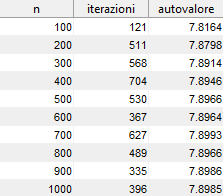
\includegraphics[scale=0.9]{cap6/6_2.png}
\end{center}

\noindent Il codice Matlab utilizzato per realizzarla \'e il seguente:

\lstinputlisting[language=Matlab]{cap6/6_2.m}
